
\chapter{Implementation}
\label{chap:implementation}
% logo definitions
\newcommand{\logoFleur}{%
  \begingroup\normalfont
  
\includegraphics[height=1.2\fontcharht\font`\B]{img/logo/fleur.png}%
  \endgroup
}
\newcommand{\logoAiida}{%
  \begingroup\normalfont
  
\includegraphics[height=1.0\fontcharht\font`\B]{img/logo/aiida.png}%
  \endgroup
}
\newcommand{\logoAiidalab}{%
  \begingroup\normalfont
  
\includegraphics[height=1.0\fontcharht\font`\B]{img/logo/aiidalab.png}%
  \endgroup
}
\newcommand{\logoBinder}{%
  \begingroup\normalfont
  
\includegraphics[height=1.2\fontcharht\font`\B]{img/logo/binder.png}%
  \endgroup
}
\newcommand{\logoBokeh}{%
  \begingroup\normalfont
  
\includegraphics[height=1.2\fontcharht\font`\B]{img/logo/bokeh.png}%
  \endgroup
}
\newcommand{\logoDash}{%
  \begingroup\normalfont
  
\includegraphics[height=1.2\fontcharht\font`\B]{img/logo/dash.png}%
  \endgroup
}
\newcommand{\logoDocker}{%
  \begingroup\normalfont
  
\includegraphics[height=1.2\fontcharht\font`\B]{img/logo/docker.png}%
  \endgroup
}
\newcommand{\logoHoloviews}{%
  \begingroup\normalfont
  
\includegraphics[height=1.2\fontcharht\font`\B]{img/logo/holoviews.png}%
  \endgroup
}
\newcommand{\logoHvplot}{%
  \begingroup\normalfont
  
\includegraphics[height=1.2\fontcharht\font`\B]{img/logo/hvplot.png}%
  \endgroup
}
\newcommand{\logoJavascript}{%
  \begingroup\normalfont
  
\includegraphics[height=1.2\fontcharht\font`\B]{img/logo/javascript.png}%
  \endgroup
}
\newcommand{\logoJupyter}{%
  \begingroup\normalfont
  
\includegraphics[height=1.2\fontcharht\font`\B]{img/logo/jupyter.png}%
  \endgroup
}
\newcommand{\logoMatplotlib}{%
  \begingroup\normalfont
  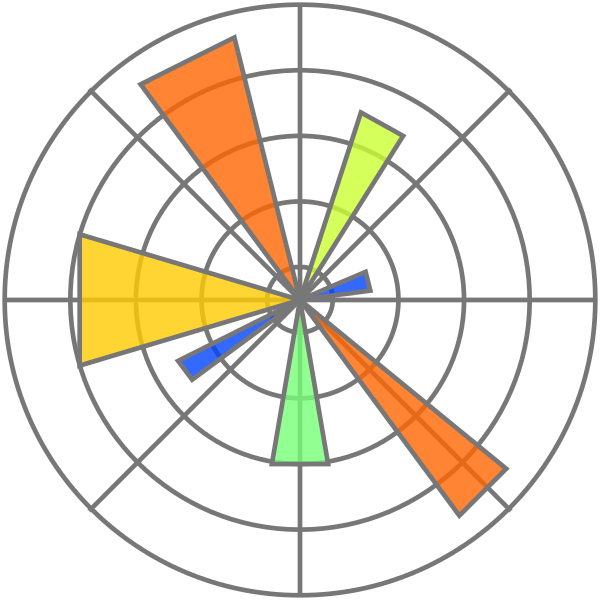
\includegraphics[height=1.2\fontcharht\font`\B]{img/logo/matplotlib.png}%
  \endgroup
}
% \newcommand{\logoMpld3}{%
%   \begingroup\normalfont
%   
\includegraphics[height=1.2\fontcharht\font`\B]{img/logo/mpld3.png}%
%   \endgroup
% }
\newcommand{\logoPanel}{%
  \begingroup\normalfont
  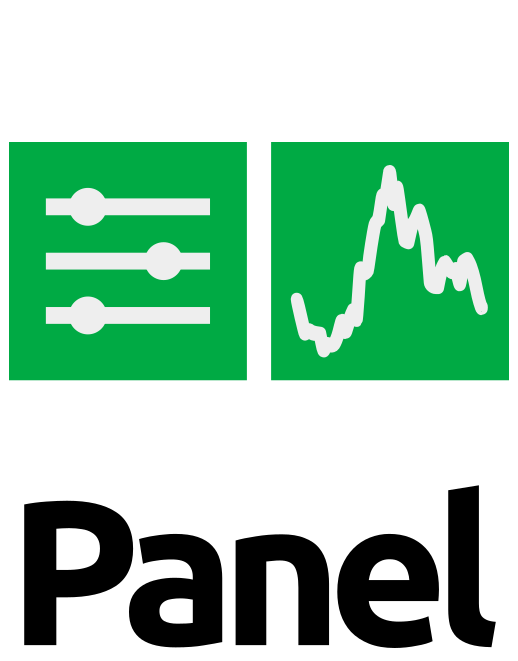
\includegraphics[height=1.2\fontcharht\font`\B]{img/logo/panel.png}%
  \endgroup
}
\newcommand{\logoParam}{%
  \begingroup\normalfont
  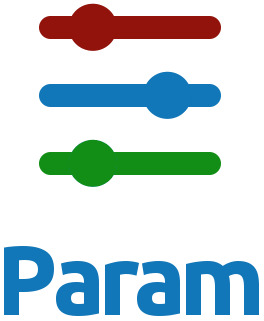
\includegraphics[height=1.2\fontcharht\font`\B]{img/logo/param.png}%
  \endgroup
}
\newcommand{\logoPlotly}{%
  \begingroup\normalfont
  
\includegraphics[height=1.2\fontcharht\font`\B]{img/logo/plotly.png}%
  \endgroup
}
\newcommand{\logoPython}{%
  \begingroup\normalfont
  
\includegraphics[height=1.2\fontcharht\font`\B]{img/logo/python.png}%
  \endgroup
}
\newcommand{\logoPyviz}{%
  \begingroup\normalfont
  
\includegraphics[height=1.2\fontcharht\font`\B]{img/logo/pyviz.png}%
  \endgroup
}
\newcommand{\logoSeaborn}{%
  \begingroup\normalfont
  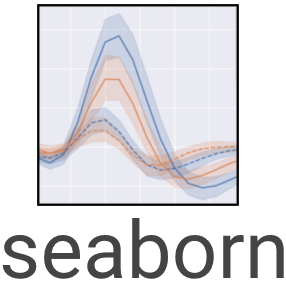
\includegraphics[height=1.2\fontcharht\font`\B]{img/logo/seaborn.png}%
  \endgroup
}

%%% Local Variables:
%%% mode: latex
%%% TeX-master: t
%%% End:


As per the requirements expounded upon in the introduction, the deliverable of
the project should be a finished software product. The software is written in
Python so as to integrate easily with the research group's ongoing software
projects around the Fleur code \cite{fleur}. These are chiefly the group's
materials science tool collection \texttt{masci-tools} \cite{masci-tools} ,
where also this project's code is hosted, and the 'Automated Interactive
Infrastructure and Database for Computational Science' (AiiDA) \cite{aiida}. The
product clients split into frontend users and code developers. In order to
accommodate this, the product is organized into three unidirectionally dependent
subpackages or -modules, see Figure \ref{fig:modules}.

An important design consideration was to account for unknown use cases. This has
been realized in each submodule by the decoupling of \textbf{interface} and
\textbf{implementation}. The interfaces do not rely on any specific input file
format, visualization method or package, unlike the implementations for a
specific task or \textbf{application}. The word 'application' in this section
denotes the band structure and density of states visualization, and for these,
implementations are provided.

This design choice was also one reason why the product does not reuse any of the
\texttt{masci-tools} routines which partly solve quite similar problems, but
seemed to be too specialized in an cursory code review. For these developers,
one added value of the project product could be to inspire the hopefully easy
integration into a common interface, where the current abstraction level could
serve as a starting point.

\begin{figure}[htb!]
    \centering
    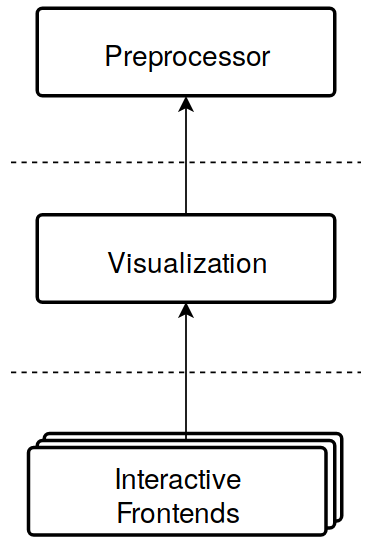
\includegraphics[width=0.3\linewidth]{img/module_design.png}
    \caption{Module Design}
    \label{fig:modules}
\end{figure}

\section{HDF Preprocessor Module}
\label{sec:preprocessor-module}

\subsection{Interface}
\label{sec:preprocessor-interface}

This is the 'backend' of the tool. It is basically a file reader for the input
data, for example a Fleur simulation output. Supported formats are the
Hierarchical Data Format (HDF) \cite{hdf} for the band structure, and a simple
Fleur-specific comma-separated values (CSV) format for the density of states
(DOS).

The HDF format is basically a binary flexible container for all kinds of common
binary and text file formats, each of which constitutes a \texttt{Dataset}
inside the HDF file. The format supports metadata annotation and high-throughput
input/output (I/O). As a consequence, it is considered by some developers in
some application domains relying on numerical simulation codes, to be one
possible base for the establishment of common domain-specific rich data exchange
standards in order to increase code interoperability. These developers are in
the process of extending their codes' I/O capabilities towards that end.
However, HDF's flexibility comes at the price of a relatively complex Application
Programming Interface (API) as the keyhole for all operations.

The preprocessor module tries to hide that complexity by offering the
\texttt{Recipes} interface, see Figure \ref{fig:preprocessor}. A specific
application \texttt{Recipe} is a dictionary that aims to describe a complete
\href{https://en.wikipedia.org/wiki/Extract,_transform,_load}{Extract-Transform-Load}
(ETL) pipeline for one specific application. The 'extract' is the reading of a
dataset from HDF, the 'transform' a sequence of once-through functions applied
to the the dataset, and the 'load' the aggregation of all transformed datasets
into one runtime object that has all the methods for operations on the data that
are going to be used later on in the intended application.

The 'transform' and 'output' type methods are defined in hierarchical
\texttt{Transform} and \texttt{Output\_Type} classes, which sort them from
general to application-specific applicability. This structure is built using
Python's \texttt{AbstractBaseClass} (\texttt{ABC}) interface. The advantages of
the 'Recipes approach' are:
\begin{itemize}
\item All ETL processes for one application are collected in one simple list
    (the recipe), not locked in different code locations with conflicting
    contexts. In this list, entries can be sorted in any manner, e.g.
    alphabetical for perusal.
\item Recipes are de/serializable (can be read from and saved to disk) and thus be
    created and manipulated by code.
\item The ETL processes declared in this way can be easily reused across
    applications. A recipe can combine different output types into a new type.
\end{itemize}

The feature that enables this flexibility is \textbf{type introspection}: the
preprocessor processes the datasets listed in the recipe in the order of their
mutual dependencies as found in the used transform and output methods. When all
transformed datasets have been added to the object, all specified output types
are searched and all their methods and attributes added. Thus the output
object's type is defined at runtime, when the preprocessing is finished.

\begin{figure}[htb!]
    \centering
    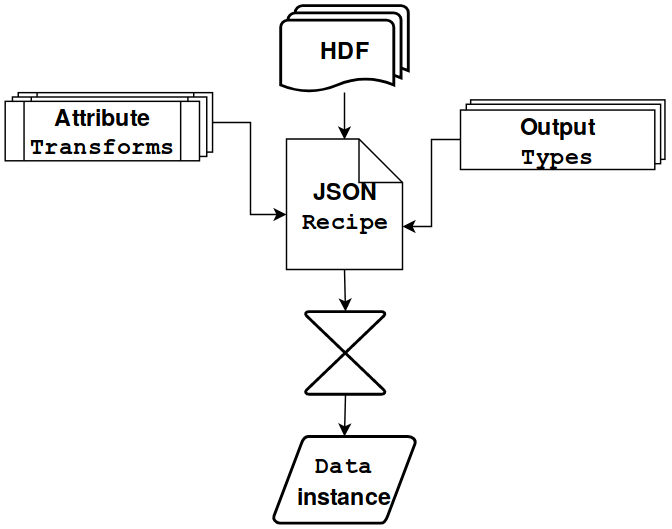
\includegraphics[width=0.6\linewidth]{img/reader_flowchart4.png}
    \caption{The preprocessor module.}
    \label{fig:preprocessor}
\end{figure}

\subsection{Implementation for Band Structure Visualization}
\label{sec:preprocessor-implementation}

\textbf{TODO} describe how bandstructure data is preprocessed for visualization
including user selections

\section{Visualization Module \& Graphical Frontends}
\label{sec:visualization-module}

\textbf{TODO} Frontends: combine into one subsection when finished. usage will
be in in user manual next section.

\subsection{Interface}
\label{sec:visualization-interface}

\textbf{TODO} describe (short!)

\begin{figure}[htb!]
    \centering
    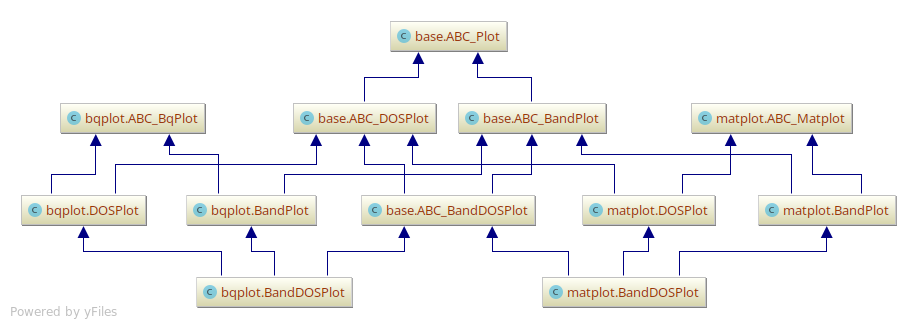
\includegraphics[width=0.8\linewidth]{img/pycharm_uml/matplot.png}
    \caption{Visualization Module Design}
    \label{fig:visualization-module}
\end{figure}

\subsection{Desktop Frontend Implementation}
\label{sec:desktop-frontend}

\subsection{Web Frontend Implementation}
\label{sec:web-frontend}

\textbf{TODO} describe tool selection process, refer to \cite{jw-notes}.




%%% Local Variables:
%%% mode: latex
%%% TeX-master: "../report"
%%% End:

%  LocalWords:  subpackages submodule
